% Compiles with pdfLaTeX + BibTeX (Overleaf default).
% Figures that show TCB prices (F2, F5) and the monitor screenshots are not in git: upload them to figures/ in Overleaf.
% Until they are there, a framed placeholder is shown instead (see \optfig below).
\documentclass[12pt]{report}

\usepackage{iftex}
\ifPDFTeX
\usepackage[T1]{fontenc}
\usepackage[utf8]{inputenc}
\usepackage{tgtermes}
\else
\usepackage{fontspec}
\setmainfont{TeX Gyre Termes}
\fi

\usepackage{graphicx}
\graphicspath{{figures/}{./}}
\usepackage{float}
\usepackage{amsmath,amssymb,amsfonts}
\usepackage{textcomp}
\usepackage[table]{xcolor}
\usepackage[hidelinks]{hyperref}
\usepackage{url}
\usepackage{ragged2e}
\usepackage{array,multirow}
\usepackage{booktabs}
\usepackage{longtable}
\usepackage{tabularx}
\usepackage{enumitem}
\usepackage{caption}
\captionsetup{font=small,labelfont=bf}
\usepackage{tikz}
\usepackage{adjustbox}
\usetikzlibrary{arrows.meta,positioning,fit,calc}

\usepackage[parfill]{parskip}
\usepackage{geometry}
\usepackage{sectsty}
\chapterfont{\centering}

\geometry{
paper=a4paper,
top=1in,
bottom=1in,
left=1.2in,
right=0.8in,
headheight=0.75cm,
footskip=1.5cm,
headsep=0.75cm,
}
\linespread{1.5}
\emergencystretch=3em

% ---------------------------------------------------------------------------
% Visible reminder for anything still to be filled in. Search the project for TODO before submitting.
\newcommand{\todo}[1]{\textbf{\textcolor{red}{[TODO: #1]}}}
\newcommand{\unexpl}{\emph{not explained by measured cost drivers}}
\newcommand{\naive}{``tomorrow = today''}
\newcommand{\retro}{\emph{(retrospective)}}
% A figure that is uploaded separately (prices or screenshots): placeholder until the file exists.
% Optional first argument: trim (left bottom right top, in image pixels) to crop blank margins of a screenshot.
\newcommand{\optfig}[3][0 0 0 0]{\IfFileExists{figures/#2}{\includegraphics[width=#3,trim=#1,clip]{#2}}{\fbox{\parbox[c][4cm][c]{#3}{\centering\textcolor{red}{Upload \texttt{figures/\detokenize{#2}} from Drive}}}}}
% Shrinks a table to the text width only if it is wider.
\newcommand{\fittab}[1]{\begin{adjustbox}{max width=\linewidth}#1\end{adjustbox}}
% A table that contains prices (built by tools/thesis_upload.py, uploaded to Overleaf, never in git): placeholder until it exists.
\newcommand{\opttab}[1]{\IfFileExists{tables/#1.tex}{\fittab{\input{tables/#1}}}{\fbox{\parbox[c][2.5cm][c]{0.8\linewidth}{\centering\textcolor{red}{Upload \texttt{tables/\detokenize{#1}.tex} (made by \texttt{tools/thesis\_upload.py})}}}}}
% Source line under a table or figure.
\newcommand{\source}[1]{\par\smallskip{\footnotesize Source: #1}}
% ---------------------------------------------------------------------------

\begin{document}

% ============================ TITLE PAGE ============================
\begin{titlepage}
\centering

\includegraphics[height=4cm,width=4cm]{unilogo.png}\par
\vspace{0.3cm}
{\huge\bfseries Comilla University \par}
\vspace{0.5cm}
{\Large\bfseries Food Price Watch: A Monitoring and Abnormal-Rise Alert System for Daily Retail Food Prices in Dhaka\par}
\vspace{0.45cm}
{\scshape\Large\bfseries A RESEARCH PROJECT REPORT \par}
{\scshape\Large\bfseries \textit{Submitted By}\par}
{\Large\textbf{MD. ROMJAN CHOWDHURY}}\par
{\Large{ID: 22408024}}\par
\vspace{0.35cm}
{\large\textbf{\textit{In Partial Fulfillment for the course Research Project of}}}\par
{\Large\textbf{MASTER OF SCIENCE (ENGINEERING)\\}}
\vspace{0.1cm}
{\large\textbf{IN }}
{\large\textbf{DEPARTMENT OF COMPUTER SCIENCE AND ENGINEERING}\par}
\vspace{0.45cm}
{\Large\textbf{COMILLA UNIVERSITY, CUMILLA-3506}}\par
\vspace{0.35cm}
{\Large\bfseries November 2026\par}
\end{titlepage}

% ============================ CERTIFICATE ============================
\newpage
\pagenumbering{gobble}
\begin{center}
\large\textbf{BONAFIDE CERTIFICATE}\\
\end{center}
\section*{}
This is to certify that this research project entitled
\textbf{``Food Price Watch: A Monitoring and Abnormal-Rise Alert System for Daily Retail Food Prices in Dhaka''}
is submitted by \textbf{Md. Romjan Chowdhury}, who carried out the project work under my supervision. This is the bonafide work.
\\
\\

\begin{table}[h]
\begin{tabular}{l@{\hspace{3cm}}l}
{Signature} & {Signature} \\
\\
\ldots\ldots\ldots\ldots\ldots\ldots\ldots\ldots & \ldots\ldots\ldots\ldots\ldots\ldots\ldots\ldots \\
Dr. Mahmudul Hasan & Dr. Mahmudul Hasan \\
\textbf{Chairman of the Exam Committee} & \textbf{Supervisor} \\
Associate Professor & Associate Professor \\
Department of CSE & Department of CSE \\
Comilla University, Cumilla. & Comilla University, Cumilla. \\
\end{tabular}
\end{table}

\pagenumbering{Roman}

% ============================ ABSTRACT ============================
\chapter*{Abstract}
\addcontentsline{toc}{chapter}{\numberline{}Abstract}
Food prices in Dhaka can rise sharply within weeks, but the daily price sheets of the Trading Corporation of Bangladesh (TCB) do not show whether a day's price is unusual. This project builds Food Price Watch, a monitoring and abnormal-rise alert system for the TCB daily retail prices of eight everyday items (broiler chicken, eggs, onion, potato, imported garlic, palm oil, soybean oil and sugar) from May 2021 to October 2026: 11,296 item-days on 1,412 report days. Each item gets an expected upper price bound for every report day, drawn one week earlier, and an alert is raised when the price is above it on 3 of the last 5 report days. Three ways of drawing the bound are compared: a range from a LightGBM forecast, a range from the forecast ``tomorrow = today'', and a fixed 7\,\% rise. Every setting was chosen on 2024 and committed before 2025-26 was scored; because an earlier run had looked at 2025-26, those results are labelled retrospective. The prices are sticky: an item's price is unchanged on 62 to 87\,\% of report days. Neither ETS nor LightGBM beats ``tomorrow = today'' at any horizon from 1 to 30 report days (relative MAE 1.01 to 1.21 in 2025-26), and every significant difference favours ``tomorrow = today''. The alerts, scored against sustained 10\,\% rises defined from the prices alone, beat the same number of alerts on random dates for every rule ($p = 0.003$): in 2025-26 the LightGBM range caught 17 of 23 sustained rises and the simple range 15 of 23, about 2.5 to 2.8 times the random-date rate, a median of 2 report days after a rise began. The two ranges catch nearly the same rises, so the monitor does not need machine learning. A Gradio app shows the status of every item on any day, its chart and a log of all alerts. The alerts detect abnormal rises that are not explained by measured cost drivers; they are not early warning.

\textbf{Keywords:} food prices, Bangladesh, price monitoring, anomaly detection, forecasting benchmark, LightGBM, prediction intervals.


% ============================ ACKNOWLEDGEMENT ============================
\chapter*{Acknowledgement}
\addcontentsline{toc}{chapter}{\numberline{}Acknowledgement}
First of all, I thank Almighty Allah for the health and patience that let me finish this project.

\noindent I am grateful to my supervisor, \textbf{Dr. Mahmudul Hasan}, Associate Professor, Department of Computer Science and Engineering, Comilla University, for his guidance and for the time he gave to this work. His questions about what the results did and did not show shaped how this report is written.

\noindent I also thank the Trading Corporation of Bangladesh, whose published daily price reports are the source of the price data, and the providers of the open data used as cost drivers: Open-Meteo for weather and the market data services behind the exchange-rate series.

\noindent Finally, I thank my family and friends for their support during this work.

% ============================ CONTENTS ============================
\newpage
\renewcommand*\contentsname{Table of Contents}
\tableofcontents
\listoffigures
\listoftables
\chapter*{List of Abbreviations}
\addcontentsline{toc}{chapter}{\numberline{}List of Abbreviations}
\begin{tabular}{ll}
ALPS & Alert for Price Spikes (World Food Programme) \\
DM & Diebold--Mariano test \\
ETS & Exponential smoothing (error, trend, seasonal) \\
FAO & Food and Agriculture Organization of the United Nations \\
HLN & Harvey--Leybourne--Newbold correction \\
LightGBM & Light Gradient Boosting Machine \\
MAE & Mean absolute error \\
MAPE & Mean absolute percentage error \\
ML & Machine learning \\
RQ & Research question \\
TCB & Trading Corporation of Bangladesh \\
Tk & Bangladeshi taka \\
WFP & World Food Programme \\
\end{tabular}

\pagenumbering{arabic}

\justifying

% ============================ CHAPTERS ============================
\chapter{Introduction}\label{ch:intro}

\section{Background}
Food takes a large share of household spending in Bangladesh, and food prices in Dhaka can rise sharply within weeks: onion, potato, eggs and broiler chicken have all had episodes in which their retail price rose by a tenth or more and stayed high. Food has a weight of about 59\,\% in the consumer price index, and food inflation was close to 14\,\% at its recent peak \cite{cpd2026}\todo{check both figures in the CPD report}.

The Trading Corporation of Bangladesh (TCB), a state agency, publishes a daily sheet of retail prices in Dhaka markets for common food items \cite{tcb}. The sheet gives, for each item, the lowest and highest price seen that day. It is public, but it is published as one document per day, so it is hard to see from it whether today's price is unusual for an item, or whether a rise is continuing.

International agencies already watch food prices for unusual movements. FAO's indicator of price anomalies compares compound growth rates of a price with their history \cite{baquedano2015}, and the World Food Programme's Alert for Price Spikes compares a price with its seasonal trend \cite{wfpalps2014}. Both are designed for monthly market prices. This project asks whether a similar kind of monitoring can be built for the daily TCB data, and whether machine learning makes it better.

\section{Motivation}
A monitor of this kind has to answer one question every day for every item: is this price unusually high for this item? A natural way to answer it is to forecast the price, draw an expected range around the forecast, and raise an alert when the price stays above the range. That raises two further questions that the literature on food price forecasting rarely asks. First, is the machine-learning forecast actually better than the simplest possible forecast, ``the price tomorrow will be the price today''? Many published studies compare complex models with each other or with ARIMA, but not with this baseline \cite{manogna2025}. Second, even if the forecast is not better, does a range built from it still make useful alerts, and are they better than alerts from a range that uses no model at all?

\section{Problem Statement}
Given the TCB daily retail prices of eight everyday food items in Dhaka from May 2021 to October 2026, build and evaluate a system that gives each item an expected price range for each report day and raises an alert when the price stays above it. The system must be evaluated honestly: every setting must be chosen on one period and scored on another, every forecast figure must be compared with \naive{}, and the alerts must be compared with what the same number of alerts on random dates would achieve.

\section{Objectives}
\begin{enumerate}[leftmargin=*,itemsep=2pt]
\item Build a clean, audited daily data table of TCB prices for eight items, with weather, exchange rate and calendar columns joined on the date they became available.
\item Describe how these prices behave and define sustained rises from the prices alone.
\item Benchmark ETS and LightGBM forecasts against \naive{} at horizons of 1 to 30 report days.
\item Build three alert rules (a range from LightGBM, a range from \naive{}, and a fixed threshold), choose their settings on 2024, and score them on 2025-26 against sustained rises and a random-date control.
\item Provide a working monitoring app that shows, for any report day, which items are in alert.
\end{enumerate}

\section{Research Questions}
\begin{table}[H]\centering\small
\caption[Research questions]{Research questions.}\label{tab:rq}
\fittab{\begin{tabularx}{\linewidth}{lXl}
\toprule
\textbf{RQ} & \textbf{Question} & \textbf{Answered in} \\
\midrule
RQ1 & How do TCB daily retail prices for the eight items behave: how often and by how much do they change, and how often do sustained rises occur? & Section~\ref{sec:res-behaviour} \\
RQ2 & Does a machine-learning or statistical forecast beat \naive{} on these prices? & Section~\ref{sec:res-forecast} \\
RQ3 & Do alerts built from an expected price range catch sustained rises more often than the same number of alerts on random dates? & Section~\ref{sec:res-alerts} \\
RQ4 & Does a range drawn from a machine-learning forecast catch more rises than a range drawn from \naive{} or a fixed threshold? & Section~\ref{sec:res-alerts} \\
\bottomrule
\end{tabularx}
}
\end{table}

\section{Scope}
The study covers eight items (broiler chicken, farm eggs, local onion, potato, imported garlic, loose palm oil, loose soybean oil and sugar), Dhaka only, from 17 May 2021 to 24 October 2026. The items were chosen after the results of an earlier, wider run of this project had been seen. The monitor replays this period; it does not collect new prices. Alerts look for abnormal \emph{rises} only. The system says that a rise is unusual; it does not say why the price rose, and a rise above the range is described only as \unexpl{}.

\section{Functionality of the System}
\begin{itemize}[leftmargin=*,itemsep=2pt]
\item Reads the TCB daily prices and the driver data, checks them and joins them into one table.
\item Computes, for each item and report day, an upper bound under each of the three rules from information available one week earlier.
\item Flags an item as in alert when its price is above the bound on 3 of the last 5 report days.
\item Shows, in a web app, the status of all items on a chosen day, a chart of each item, and a log of every alert.
\end{itemize}

\section{Contributions}
\begin{enumerate}[leftmargin=*,itemsep=2pt]
\item An audited daily data table for eight items from the TCB reports, with drivers joined on their availability dates and the sparse 2022 period kept as a gap.
\item A forecast benchmark in which every figure is shown next to \naive{} and every setting was committed before scoring; it finds that neither ETS nor LightGBM beats \naive{}.
\item A comparison of three alert rules against a model-free definition of a sustained rise, with a random-date control; all three beat random dates, and the range from \naive{} catches the same rises as the range from LightGBM.
\item A working monitoring app built on these rules.
\end{enumerate}

\section{Organization of the Report}
Chapter~\ref{ch:lit} reviews related work. Chapter~\ref{ch:method} describes the data, the cleaning, the forecast benchmark, the alert rules and how they are evaluated. Chapter~\ref{ch:results} gives the results and discusses them. Chapter~\ref{ch:concl} answers the research questions and lists limitations and future work. The appendices give the reproducibility record, the results register and the changes made to the original plan.

\chapter{Literature Review}\label{ch:lit}
% Written from the abstracts of the papers. The student reads each paper before submission (reports/thesis/READING_LIST.md).

\section{Related Works}

\subsection{Food price monitoring and alert indicators}
Two indicators are used internationally to flag unusual food prices. Baquedano \cite{baquedano2015} developed, for FAO's Global Information and Early Warning System, an indicator of price anomalies based on a weighted combination of quarterly and annual compound growth rates, each compared with its own historical mean and spread; it became the basis of the SDG indicator 2.c.1. The World Food Programme's Alert for Price Spikes (ALPS) compares a market price with its estimated seasonal trend and grades the difference into alert levels \cite{wfpalps2014}. Both work on monthly prices across many markets. Neither forecasts with machine learning; both define ``unusual'' from the series' own history. This project does the same on daily data and tests whether a forecast-based range improves on that.

\subsection{How retail prices change}
Studies of individual retail prices find that prices change infrequently and stay fixed for weeks or months between changes \cite{klenow2010,nakamura2008}. Cavallo \cite{cavallo2018} showed with daily prices collected online that price spells are long and that very small changes are rare, and that some earlier findings came from how prices had been sampled. These findings explain the stickiness found in the TCB data and why ``no change'' is a strong forecast for it.

\subsection{Forecasting food and agricultural prices}
Machine learning is widely used to forecast food prices. Ogol et al.\ \cite{ogol2025} forecast Kenyan food prices from WFP data with a hybrid of gradient-boosting models and deployed it as a web application. Manogna et al.\ \cite{manogna2025} compared ARIMA, support vector regression, XGBoost and several neural networks on daily wholesale prices of 23 Indian commodities and found recurrent networks most accurate; the comparison does not include a no-change forecast. For Bangladesh, Jubayer et al.\ \cite{jubayer2024} studied the growth and instability of onion production and forecast onion prices with time-series models, and Mila et al.\ \cite{onionnardl} studied how onion prices are transmitted between markets\todo{check method details in both papers}. Closest to this project, Muhammad et al.\ \cite{agripricebd} built a daily dataset of Bangladeshi retail prices from government reports and compared classical and deep-learning models; naive persistence was best on commodities that behave like a random walk.

\subsection{Benchmarks and forecast evaluation}
A forecast is only useful if it beats a simple benchmark. Meese and Rogoff \cite{meese1983} found that structural exchange-rate models did not beat a random walk out of sample, a result that has made the random walk a standard benchmark. The M5 competition \cite{makridakis2022} evaluated many methods on retail sales with common error measures. Hyndman and Koehler \cite{hk2006} recommend scale-free measures relative to a naive forecast. Differences in accuracy are tested with the Diebold--Mariano test \cite{dm1995} and its small-sample correction \cite{hln1997}, and many tests at once are corrected with the Holm procedure \cite{holm1979}. The ETS candidate follows the state-space framework of Hyndman et al.\ \cite{hyndman2002}, and the machine-learning candidate is LightGBM \cite{lightgbm}.

\subsection{Ranges from forecast errors}
An expected range can be built from a model's own past out-of-sample errors instead of from its assumptions; Lee and Scholtes \cite{lee2014} studied such empirical prediction intervals. Whether a range holds the stated share of observations can be tested with Kupiec's coverage test \cite{kupiec}, developed for value-at-risk models.

\section{Summary of Related Works}
\begin{table}[H]\centering\small
\caption[Summary of related works]{Summary of related works.}\label{tab:litsum}
\begin{tabularx}{\linewidth}{>{\raggedright\arraybackslash}p{2.6cm}>{\raggedright\arraybackslash}p{3.2cm}>{\raggedright\arraybackslash}p{3.0cm}X}
\toprule
\textbf{Work} & \textbf{Data} & \textbf{Method} & \textbf{Relevance / gap} \\
\midrule
Baquedano \cite{baquedano2015} & monthly food prices, many countries & compound growth rate anomaly & monthly; no forecast \\
WFP ALPS \cite{wfpalps2014} & monthly market prices & deviation from seasonal trend & monthly; no forecast \\
Ogol et al.\ \cite{ogol2025} & Kenyan food prices (WFP) & gradient-boosting hybrid, web app & no alert rules \\
Manogna et al.\ \cite{manogna2025} & daily wholesale, 23 Indian commodities & ARIMA, ML, deep learning & no naive benchmark \\
Jubayer et al.\ \cite{jubayer2024} & Bangladesh onion & time-series forecast & one item; no alerts \\
Muhammad et al.\ \cite{agripricebd} & daily Bangladeshi retail prices & classical and deep models & naive wins on random-walk items; no alerts \\
Klenow and Malin \cite{klenow2010}, Cavallo \cite{cavallo2018} & retail micro prices & descriptive & prices are sticky \\
This work & TCB daily Dhaka prices, 8 items & naive, ETS, LightGBM; three alert rules & alerts scored against model-free rises and random dates \\
\bottomrule
\end{tabularx}
\end{table}

\section{Research Gap}
The works above leave three gaps that this project addresses. First, the established price-anomaly indicators work on monthly prices; there is no tested daily monitor for Dhaka retail prices. Second, many machine-learning studies of food prices do not report a no-change benchmark, so it is not known whether their models would beat it on sticky retail prices. Third, studies that forecast prices rarely ask whether a forecast-based alert is better than an alert that needs no model, or test their alerts against chance.

\section{Contributions}
This project builds a daily monitor for eight TCB items, benchmarks two forecasting methods against \naive{} with settings committed before scoring, and compares three alert rules against a model-free definition of a sustained rise and a random-date control (Section~1.8).

\chapter{Methodology}\label{ch:method}

This chapter describes the data, how it was cleaned and joined, the reference that alerts are scored against, the forecast benchmark, the three alert rules, and how every setting was chosen and then scored. The whole pipeline is shown in Figure~\ref{fig:workflow}. Each step is one Jupyter notebook; the code is in a public GitHub repository and the data, which contains TCB prices, stays in a private Google Drive folder.

\begin{figure}[H]
\centering
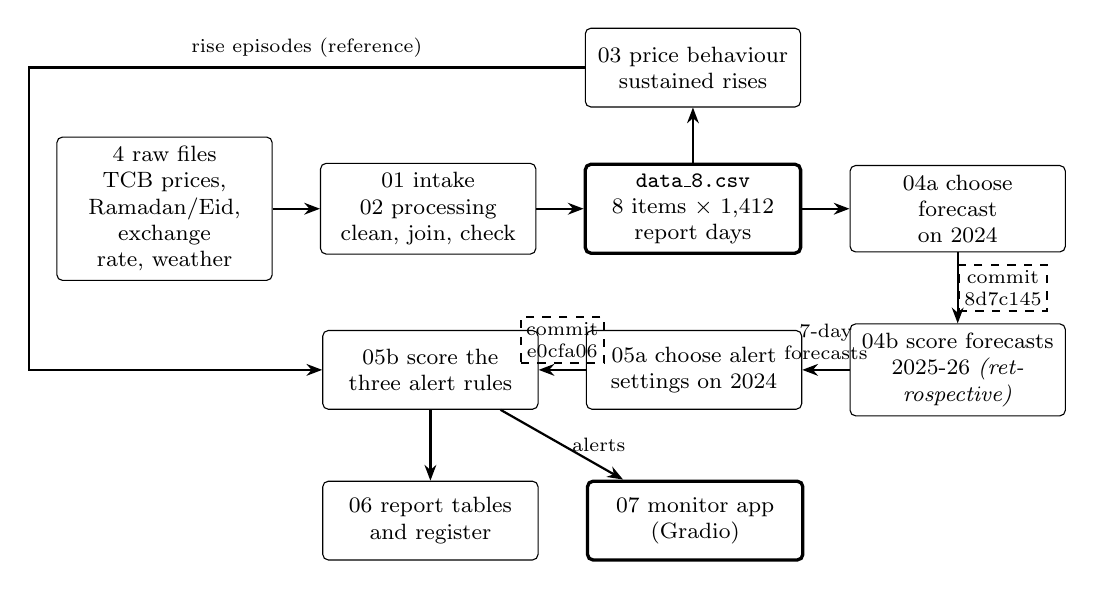
\begin{tikzpicture}[
  box/.style={draw, rounded corners=2pt, align=center, font=\footnotesize, minimum height=1.0cm, text width=2.5cm},
  key/.style={box, very thick},
  gate/.style={draw, dashed, font=\scriptsize, align=center, inner sep=2pt},
  arr/.style={-{Stealth[length=2mm]}, thick},
  lab/.style={font=\scriptsize, align=center}]
\node[box] (raw) {4 raw files\\TCB prices, Ramadan/Eid,\\exchange rate, weather};
\node[box, right=0.6cm of raw] (n02) {01 intake\\02 processing\\clean, join, check};
\node[key, right=0.6cm of n02] (data) {\texttt{data\_8.csv}\\8 items $\times$ 1,412\\report days};
\node[box, above=0.7cm of data] (n03) {03 price behaviour\\sustained rises};
\node[box, right=0.6cm of data] (n04a) {04a choose forecast\\on 2024};
\node[box, below=0.9cm of n04a] (n04b) {04b score forecasts\\2025-26 \retro};
\node[box, left=0.6cm of n04b] (n05a) {05a choose alert\\settings on 2024};
\node[box, left=0.6cm of n05a] (n05b) {05b score the\\three alert rules};
\node[box, below=0.9cm of n05b] (n06) {06 report tables\\and register};
\node[key, right=0.6cm of n06] (n07) {07 monitor app\\(Gradio)};
\draw[arr] (raw) -- (n02);
\draw[arr] (n02) -- (data);
\draw[arr] (data) -- (n03);
\draw[arr] (data) -- (n04a);
\draw[arr] (n04a) -- node[gate, right] {commit\\8d7c145} (n04b);
\draw[arr] (n04b) -- node[lab, above] {7-day\\forecasts} (n05a);
\draw[arr] (n05a) -- node[gate, above=2pt] {commit\\e0cfa06} (n05b);
\coordinate (L) at ($(raw.west)+(-0.35,0)$);
\draw[arr] (n03.west) -- node[lab, above] {rise episodes (reference)} (n03.west -| L) |- (n05b.west);
\draw[arr] (n05b) -- (n06);
\draw[arr] (n05b) -- node[lab, right] {alerts} (n07);
\end{tikzpicture}
\caption[Workflow of Food Price Watch]{Workflow of Food Price Watch. Each box is one notebook. The dashed labels are commits: a setting chosen on 2024 was written into the settings file and pushed before the notebook that scores 2025-26 was run.}
\label{fig:workflow}
\end{figure}

\section{Data}\label{sec:data}

\subsection{Sources}
The prices come from the daily retail price reports of the Trading Corporation of Bangladesh (TCB) for Dhaka \cite{tcb}. On most working days TCB publishes a sheet that gives, for each item, the lowest and highest retail price seen in Dhaka markets that day, in taka. The sheets from 17 May 2021 to 24 October 2026 had been converted into one long table during an earlier phase of this work and checked against the original files: a machine re-read of 1,530 sampled rows on 28 report days compared 3,060 price cells and found no mismatch. The audit checks the copying only; it cannot show that TCB itself recorded a value correctly.

Three other files are used: Ramadan and Eid dates; the taka per US dollar exchange rate (daily market quotes); and daily weather at 13 locations in Bangladesh from Open-Meteo \cite{openmeteo}. The four raw files are copied once into a \texttt{raw/} folder, never edited, and listed with their sha256 hashes in a manifest.

\subsection{The eight items}
The study covers eight everyday items (Table~\ref{tab:items}). They were chosen because they are common household purchases and because their prices move often enough to study. They were chosen after the results of an earlier, wider run of this project (54 items) had been seen; this is a limitation and is discussed in Section~\ref{sec:threats}. Each item is a product together with its unit, for example eggs per hali (four eggs). The group names come from the earlier run and are used only to describe the items.

\begin{table}[H]\centering\small
\caption[The eight items]{The eight items, their units, groups, the cost drivers used for each, and the share of report days on which the price is missing.}\label{tab:items}
\begin{tabular}{llllr}
\toprule
\textbf{Item} & \textbf{Unit} & \textbf{Group} & \textbf{Drivers used} & \textbf{Not reported (\%)} \\
\midrule
Chicken - Broiler & per kg & volatile perishable & none & 0.00 \\
Egg - Farm & per hali (4 pcs) & volatile perishable & none & 0.07 \\
Onion - Local & per kg & volatile perishable & weather & 0.07 \\
Potato & per kg & domestic staple & weather & 0.07 \\
Garlic - Imported & per kg & imported staple & exchange rate & 0.07 \\
Palm Oil - Loose & per litre & administered & exchange rate & 0.00 \\
Soybean Oil - Loose & per litre & administered & exchange rate & 0.28 \\
Sugar & per kg & administered & exchange rate & 0.00 \\
\bottomrule
\end{tabular}

\source{\path{reports/tables/report/R1_data.csv} (notebook 02).}
\end{table}

\subsection{Data format and shape}
Everything is joined into one table, \texttt{data\_8.csv}, in long format: one row per item and report day. With 8 items and 1,412 report days it has 11,296 rows and 20 columns and no duplicate keys (Table~\ref{tab:columns}). Lags, rolling means and forecast targets depend on the forecast horizon, so they are built from the price inside the forecasting notebooks instead of being stored.

\begin{table}[H]\centering\small
\caption[Columns of the data table]{Columns of \texttt{data\_8.csv}.}\label{tab:columns}
\begin{tabularx}{\linewidth}{>{\raggedright\arraybackslash}p{5.2cm}X}
\toprule
\textbf{Column(s)} & \textbf{Meaning} \\
\midrule
\texttt{Date}, \texttt{item\_id} & report day; item as ``product $|$ unit'' (the key) \\
\texttt{Price\_Min}, \texttt{Price\_Max}, \texttt{Price\_Avg} & lowest and highest Dhaka retail price in the TCB sheet and their midpoint (Tk); blank = not reported \\
\texttt{report\_idx} & report-day number, 0 = 17 May 2021; the time axis for lags and horizons \\
\texttt{gap\_2022} & the day lies in the sparse 2022 period \\
\texttt{days\_since\_prev\_report} & calendar days since the previous TCB sheet \\
\texttt{reports\_since\_change} & report days the price has stayed the same \\
\texttt{month}, \texttt{dow}, \texttt{days\_to\_ramadan}, \texttt{days\_to\_eid\_fitr}, \texttt{days\_to\_eid\_adha}, \texttt{in\_ramadan} & calendar, known in advance \\
\texttt{wx\_tmax\_7d}, \texttt{wx\_tmean\_30d}, \texttt{wx\_rain\_7d} & 7-day maximum temperature, 30-day mean temperature, 7-day rainfall (Bangladesh mean); onion and potato only \\
\texttt{fx\_lvl}, \texttt{fx\_ch30} & log taka per US dollar and its 30-day change; garlic, both oils and sugar only \\
\bottomrule
\end{tabularx}

\end{table}

\subsection{Cleaning rules}
The cleaning follows a small set of fixed rules. None of them invents a price, removes a real one, or uses a value before it was known.
\begin{enumerate}[leftmargin=*,itemsep=2pt]
\item \textbf{Price.} The price of an item on a day is the midpoint $P = (P_{\min} + P_{\max})/2$. TCB reports whole taka, so the midpoint moves in steps of Tk 0.5; every observed change is a multiple of 0.5.
\item \textbf{Missing prices.} A blank or zero price means ``not reported''. This affects 8 of the 11,296 cells. A missing price is never filled in a forecast target and never counted as a zero change. Model inputs may carry the last reported price forward.
\item \textbf{The 2022 gap.} From 12 March to 31 December 2022 TCB published only 24 sheets. These rows are kept and flagged. No price change, rise window, forecast target or model fit spans the gap, and ETS is fitted on data after the gap only.
\item \textbf{Real jumps stay.} There is no outlier removal: a jump in a TCB sheet is exactly what the alerts are meant to see.
\item \textbf{Checks.} Notebook 02 stops if any of these fails: duplicate keys; a midpoint that is not the average of minimum and maximum; minimum above maximum; a zero, negative or infinite price; a driver used before it was available; a driver attached to an item that does not use it.
\end{enumerate}

\subsection{Cost drivers and availability dates}\label{sec:avail}
Two clocks are used. Horizons and lags count \emph{report days}, because TCB does not publish every calendar day: ``seven days ahead'' means seven TCB sheets ahead. Drivers are joined by the \emph{calendar date on which they became known}:
\begin{itemize}[leftmargin=*,itemsep=2pt]
\item Weather of day $d$ is treated as usable from day $d+5$.
\item The exchange rate on a report day is the last quote on or before that day. Its 30-day change uses the last quote on or before the day 30 days earlier. A quote older than 7 days is left empty, never set to zero.
\item Calendar columns (month, weekday, days to Ramadan and the two Eids) are known in advance and may be used at any time.
\end{itemize}
Weather is used only for onion and potato, and the exchange rate only for imported garlic, the two oils and sugar (Table~\ref{tab:items}).

\section{Price behaviour and sustained rises}\label{sec:method-behaviour}

\subsection{Price-change measures}
For each item, notebook 03 measures how often the price changes from one report day to the next, the size of the changes when they happen, how long the price stays unchanged, the smallest price step, and whether prices behave differently in the 30 days before Ramadan. These measures are descriptive. They explain why forecasting these prices is hard, and they say nothing about why prices move.

\subsection{Sustained rise: the reference for scoring alerts}\label{sec:rise}
An alert has to be scored against something that does not depend on any model. The reference is a \emph{sustained rise}, defined from TCB prices alone:
\begin{enumerate}[leftmargin=*,itemsep=2pt]
\item On each report day $t$ the rise ratio is $R_t = P_t / P_{t-14} - 1$, where $t-14$ is 14 report days earlier. Windows that touch the 2022 gap are skipped.
\item Day $t$ is a \emph{rise day} if $R_t \geq 10\,\%$.
\item A \emph{sustained rise episode} is a run of at least 5 consecutive rise days. Episodes of the same item fewer than 14 report days apart are merged. The first rise day is the \emph{onset}.
\end{enumerate}
This rule was fixed in the earlier run before this study started and was not re-chosen. The same counts with 7\,\% and 15\,\% thresholds are reported as a sensitivity check and are never used to choose anything.

\section{Forecast benchmark}\label{sec:method-forecast}
The forecasts are a benchmark: they test whether a model can say something about the next days that \naive{} cannot. Every model forecasts the change in the logarithm of the price over $h$ report days, $y_{t,h} = \log P_{t+h} - \log P_t$, for $h \in \{1, 7, 14, 30\}$. Working in log changes puts an item that costs Tk 20 and one that costs Tk 200 on the same scale.

\subsection{Models}
\begin{itemize}[leftmargin=*,itemsep=2pt]
\item \textbf{Naive (\naive).} The forecast change is zero: the last reported price.
\item \textbf{ETS.} Automatic exponential smoothing \cite{hyndman2002}, fitted to each item's log price after the 2022 gap with the AutoETS function of statsforecast \cite{statsforecast}.
\item \textbf{LightGBM.} One gradient-boosted tree model \cite{lightgbm} for all items and all four horizons, with the horizon as an input. The price-history inputs are the log changes over the last 1, 7, 14 and 30 report days, the deviation of the price from its 30-report mean, the 30-report volatility of daily changes, the number of report days since the price last changed, and the item. The ``price plus drivers'' feature set adds the calendar, weather and exchange-rate columns.
\end{itemize}

\subsection{Training, validation and test}\label{sec:splits}
The data is never shuffled. A forecast is made at a \emph{forecast origin}, and a model fitted for that origin sees only rows whose target lies on or before the origin. The training window expands as time moves on (Figure~\ref{fig:splits}).
\begin{itemize}[leftmargin=*,itemsep=2pt]
\item \textbf{Training:} all history before each origin.
\item \textbf{Validation:} the year 2024, 43 weekly origins. Every choice of model setting, alert level and threshold is made here.
\item \textbf{Test:} 1 January 2025 to 24 October 2026, 82 weekly origins whose 30-day targets all fall on or before the last report day. This period had already been looked at in the earlier run of the project, so its results are called \emph{retrospective} throughout.
\end{itemize}
Origins are 7 report days apart. LightGBM is refitted every 8 origins and reused in between; ETS is refitted at every origin.

\begin{figure}[H]
\centering
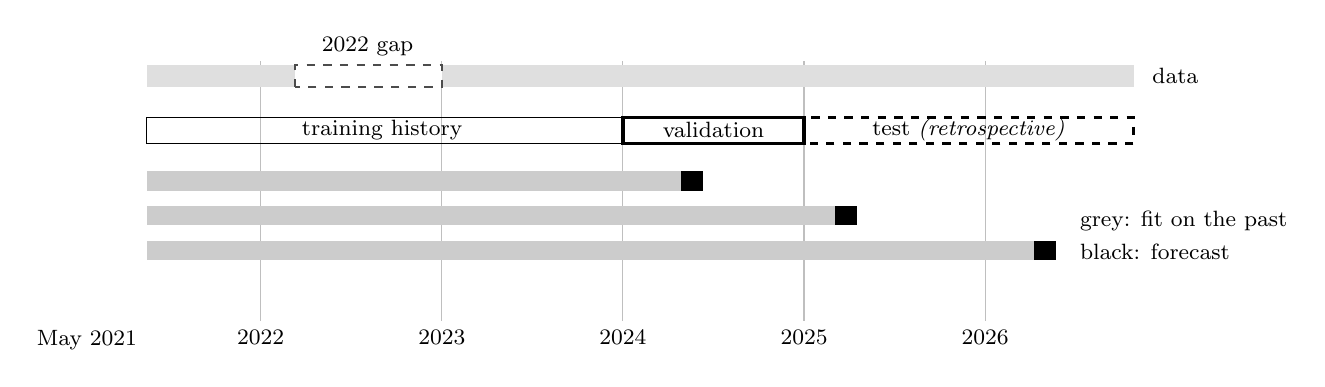
\begin{tikzpicture}[x=2.3cm, y=0.55cm, font=\footnotesize]
\foreach \yr/\x in {2022/0.63, 2023/1.63, 2024/2.63, 2025/3.63, 2026/4.63}{
  \draw[gray!50] (\x,-0.4) -- (\x,5.6); \node[below] at (\x,-0.4) {\yr};}
\node[below left] at (0,-0.4) {May 2021};
\fill[gray!25] (0,5) rectangle (5.45,5.5);
\fill[white] (0.82,5) rectangle (1.63,5.5);
\draw[thick, black!70, dashed] (0.82,5) rectangle (1.63,5.5);
\node[right] at (5.5,5.25) {data};
\node[above] at (1.22,5.5) {2022 gap};
\draw (0,3.7) rectangle (2.63,4.3); \node at (1.3,4) {training history};
\draw[very thick] (2.63,3.7) rectangle (3.63,4.3); \node at (3.13,4) {validation};
\draw[very thick, dashed] (3.63,3.7) rectangle (5.45,4.3); \node at (4.54,4) {test \retro};
\foreach \e/\yy in {2.95/2.6, 3.8/1.8, 4.9/1.0}{
  \fill[gray!40] (0,\yy) rectangle (\e,\yy+0.45);
  \fill[black] (\e,\yy) rectangle (\e+0.12,\yy+0.45);}
\node[right] at (5.1,1.9) {grey: fit on the past};
\node[right] at (5.1,1.2) {black: forecast};
\end{tikzpicture}
\caption[Training, validation and test periods]{Training, validation and test periods. The grey bars show three example forecast origins: the model is fitted on everything before the origin and forecasts the next 1 to 30 report days. The 2022 gap is never crossed.}
\label{fig:splits}
\end{figure}

\subsection{Choosing the LightGBM setting}
Sixteen configurations were compared on 2024: feature set (price only; price plus drivers) $\times$ number of leaves (7; 31) $\times$ learning rate (0.03; 0.05) $\times$ loss (absolute error; Huber), with 300 boosting rounds. The score is the geometric mean, over items and horizons, of the model's MAE divided by the MAE of \naive{}. Configurations were ordered from simplest to most complex, and a simpler one within 1\,\% of the best was preferred. The chosen setting was written into the settings file and committed (commit \texttt{8d7c145}) before the test notebook was written.

\section{The alert system}\label{sec:method-alerts}
The monitor compares each day's price with an \emph{expected range} drawn 7 report days earlier and raises an alert when the price stays above that range. It is abnormal-rise detection: it says that a rise is unusual for that item, not that a rise is coming.

\subsection{The expected range}
Every report day since June 2023 has a 7-report-ahead forecast. For target day $t$, the forecast was made at origin $t-7$. The upper bound adds to that forecast the $q$-quantile of the item's last 120 forecast errors whose targets lay on or before the origin $t-7$. Only errors that were already known at the origin are used, so the range never looks ahead. At least 30 known errors are needed before a range is drawn. This way of building a range from past out-of-sample errors follows Lee and Scholtes \cite{lee2014}.

\subsection{Three rules}
The three rules differ only in how the upper bound is drawn (Table~\ref{tab:rules}). Rule A uses the LightGBM forecast and its errors. Rule B uses \naive{}, so its errors are simply the item's past 7-report price changes. Rule C uses no model at all: it is a fixed percentage rise over 7 report days, the same for every item.

\begin{table}[H]\centering\small
\caption[The three alert rules]{The three alert rules and their candidate settings.}\label{tab:rules}
\begin{tabularx}{\linewidth}{lXl}
\toprule
\textbf{Rule} & \textbf{Upper bound on report day $t$} & \textbf{Candidates} \\
\midrule
A. ML range & LightGBM forecast of the 7-report change made at $t-7$, plus the $q$-quantile of the item's last 120 known LightGBM errors & $q \in \{0.90, 0.95, 0.975, 0.99\}$ \\
B. Simple range & ``no change'' made at $t-7$, plus the $q$-quantile of the item's last 120 known 7-report changes & $q \in \{0.90, 0.95, 0.975, 0.99\}$ \\
C. Fixed rise & price at $t-7$ times $(1+c)$, the same $c$ for every item & $c \in \{3, 5, 7, 10\}\,\%$ \\
\bottomrule
\end{tabularx}

\end{table}

\subsection{From exceedance to alert}
A day is an \emph{exceedance} when the price is above the upper bound. A single exceedance is not an alert: one-day jumps are common and often reverse. An item is in \emph{alert} on day $t$ when it exceeded the bound on at least 3 of its last 5 report days. Consecutive alert days form one \emph{alert run}, and the first day of the run is the day the monitor would report.

\subsection{Choosing the settings on 2024}
For each rule, the candidate settings were scored on 2024. The chosen setting is the most sensitive one whose alert runs that match no sustained rise stay at or below 2 per item-year, where an item-year is 250 report days. The three settings were committed (commit \texttt{e0cfa06}) before the scoring notebook was written.

\section{Evaluation}\label{sec:eval}

\subsection{Forecast accuracy}
\begin{itemize}[leftmargin=*,itemsep=2pt]
\item \textbf{MAE} of the log change, and the MAE of \naive{} on the same targets.
\item \textbf{Relative MAE} = model MAE / \naive{} MAE, combined over items with a geometric mean \cite{hk2006}. Below 1 is better than \naive{}.
\item \textbf{Accuracy} = $1 - $ MAPE. It is shown only next to the accuracy of \naive{}: on prices that rarely move, a high accuracy costs nothing.
\item \textbf{Diebold--Mariano test} \cite{dm1995} with the small-sample correction of Harvey, Leybourne and Newbold \cite{hln1997}, on the per-origin loss difference against \naive{}. The eight model--horizon $p$-values of a period are corrected with the Holm method \cite{holm1979}.
\end{itemize}

\subsection{Alert scoring}
An alert run is \emph{matched} to a sustained rise of the same item if it starts between 14 report days before the onset and 7 report days after the end of the episode. Each episode can be matched by at most one run and each run by at most one episode.
\begin{itemize}[leftmargin=*,itemsep=2pt]
\item \textbf{Recall:} share of sustained rises with a matched alert run.
\item \textbf{Precision:} share of alert runs that match a sustained rise.
\item \textbf{Median delay:} report days from the onset of a rise to the start of its matched run.
\item \textbf{Unmatched runs per item-year:} the cost side, used to choose the settings.
\item \textbf{Random-date control:} for each item, its alert runs are shifted to random positions within the period, keeping their number and spacing, and the recall is recomputed; this is repeated 300 times. The $p$-value is $(1 + \text{number of draws at least as good as the real recall}) / 301$, so the smallest possible value is $0.003$.
\item \textbf{Range coverage:} share of days on which the price was at or below the upper bound, against the nominal level, with Kupiec's test \cite{kupiec}.
\end{itemize}

\section{The monitoring app}\label{sec:method-monitor}
Notebook 07 builds one row per item and report day from 13 June 2023 to 24 October 2026 (8,432 rows): the price, the upper bound of each rule in taka, and the exceedance, alert and run-start flags. A check confirms that its alert flags are identical to those scored in notebook 05b. A Gradio app \cite{gradio} then shows four views: the status of every item on a chosen day, a chart of one item with its bounds and alerts, a log of every alert run, and a page that explains the rules and the results. Everything shown for a day uses only information known on that day. The app replays the data to 24 October 2026; it does not fetch new prices.

\section{Reproducibility}
Each notebook starts by cloning the code from GitHub and prints the code commit and the sha256 hashes of its inputs and outputs. Tables in the repository contain only rates and counts; files that contain prices stay on Drive because TCB states no reuse terms. Every headline number in this report is listed with its table, notebook and commit in a results register (Appendix~\ref{app:register}).

\chapter{Experiments and Results}\label{ch:results}

The results are given in the order of the research questions: how the prices behave (RQ1), whether any forecast beats \naive{} (RQ2), and whether the alerts catch sustained rises, and which rule does so best (RQ3, RQ4). Results for 2024 are validation results, on which every setting was chosen. Results for 2025-26 are \emph{retrospective}: no setting was chosen on them, but that period had been looked at in an earlier run of this project.

\section{Experimental Setup}

\subsection{Hardware and software}
\begin{table}[H]\centering\small
\caption[Hardware]{Hardware used.}\label{tab:hardware}
\fittab{\begin{tabular}{lp{9cm}}
\toprule
\textbf{Component} & \textbf{Details} \\
\midrule
Work computer & Windows 10; data conversion and audit, code, local runs while Google Drive could not be mounted in Colab \\
Runs of record & Google Colab, CPU runtime, no GPU \\
Storage & Google Drive folder for data and outputs; public GitHub repository for code and summary tables (no prices) \\
\bottomrule
\end{tabular}
}
\end{table}

\begin{table}[H]\centering\small
\caption[Software]{Software used.}\label{tab:software}
\fittab{\begin{tabular}{lp{8.5cm}}
\toprule
\textbf{Tool} & \textbf{Use} \\
\midrule
Python (Colab) & all notebooks \\
pandas, NumPy & data table, features, scoring \\
LightGBM ($\geq$ 4.3) \cite{lightgbm} & machine-learning forecast \\
statsforecast ($\geq$ 2.0) \cite{statsforecast} & ETS forecast (AutoETS) \\
Matplotlib & figures \\
Gradio 5 \cite{gradio} & monitoring app \\
Git, GitHub & code versions; settings committed before scoring \\
\bottomrule
\end{tabular}
}
\end{table}

\subsection{Implementation details}
The system is written in Python as a small package, \texttt{foodwatch}, that the notebooks call; each notebook does one task (Table~\ref{tab:modules}). The notebooks are generated from one script so that their setup cells are identical: they mount Google Drive, clone the code from the \texttt{main} branch of GitHub, and set the data folder. Settings are read from \path{config/settings.yaml}, and each notebook ends by printing a summary with its checks, so that a run can be confirmed from its last cell.

\begin{table}[H]\centering\small
\caption[Code modules and notebooks]{Code modules and notebooks.}\label{tab:modules}
\begin{tabularx}{\linewidth}{>{\raggedright\arraybackslash}p{4.3cm}X}
\toprule
\textbf{File} & \textbf{Role} \\
\midrule
\texttt{paths.py}, \texttt{load.py} & data folder, settings, readers for the four raw files, hashing \\
\texttt{panel.py}, \texttt{features.py}, \texttt{checks.py} & item $\times$ report-day rows, drivers joined on availability date, data checks \\
\texttt{behaviour.py} & price-change measures and sustained rise episodes \\
\texttt{forecast.py}, \texttt{metrics.py} & naive, ETS and LightGBM on an expanding window; MAE, relative MAE, Diebold--Mariano with Holm \\
\texttt{alerts.py} & ranges from known errors, the three rules, persistence, matching, random-date control, Kupiec test \\
\texttt{monitor.py}, \texttt{app/monitor\_app.py} & day-by-day monitor table and the Gradio app \\
\texttt{report.py} & report tables, figures and the results register \\
notebooks 01--07 & intake, processing, price behaviour, forecast choice and test, alert choice and scoring, report tables, monitor \\
\texttt{tools/} & notebook generator; TCB conversion and audit scripts; thesis files with prices for Overleaf \\
\bottomrule
\end{tabularx}
\end{table}

\subsection{Runs}
Notebooks 01 to 06 were first run on the work computer, while Google Drive could not be mounted in Colab, and then again in Google Colab once it could. Every output file of the Colab runs was byte-identical to the local run (same sha256 hashes); the Colab runs are the runs of record. Each run, its code commit and its file hashes are logged in \path{reports/RUN_LOG.md}.

\section{Dataset}
The data table has 11,296 rows: 8 items on 1,412 report days from 17 May 2021 to 24 October 2026. Prices are missing on 0 to 0.28\,\% of report days per item (Table~\ref{tab:items}). The 2022 gap holds 24 report days. The audit of the converted TCB sheets found no mismatch in 3,060 price cells. Table~\ref{tab:periods} shows how the data is divided in time.

\begin{table}[H]\centering\small
\caption[Distribution of the data over the periods]{Distribution of the data over the periods. Forecasts are per model and horizon; rises are sustained 10\,\% rises by onset date.}\label{tab:periods}
\begin{adjustbox}{max width=\linewidth}\begin{tabular}{lrrrrr}
\toprule
\textbf{Period} & \textbf{Report days} & \textbf{Item-days} & \textbf{Origins} & \textbf{Forecasts} & \textbf{Rises} \\
\midrule
History (May 2021 -- 2023), training only & 480 & 3,840 & -- & -- & 36 \\
2024 validation & 329 & 2,632 & 43 & 344 & 11 \\
2025 -- Oct 2026 test \retro & 603 & 4,824 & 82 & 656 & 23 \\
\midrule
All & 1,412 & 11,296 & 125 & 1,000 & 70 \\
\bottomrule
\end{tabular}\end{adjustbox}
\end{table}


\section{Price Behaviour (RQ1)}\label{sec:res-behaviour}

\subsection{Prices rarely change}
On most report days an item's price is the same as on the previous report day: from 62\,\% of days for broiler chicken to 87\,\% for sugar. Over the whole period the price changed on 12.6\,\% (sugar) to 37.5\,\% (chicken) of report days, and less often in 2024-26 than before (Table~\ref{tab:behaviour}, Figure~\ref{fig:f1}). When a price does change, the typical change is small for the administered items (about 1\,\% for the two oils) and larger for perishables (5\,\% for onion, 6.25\,\% for potato). A price can stay unchanged for long stretches: up to 104 report days for sugar and 102 for palm oil.

\begin{table}[H]\centering\small
\caption[How often and how much prices change]{How often and how much prices change. Change sizes are on days the price changed; unchanged runs are in report days; the last column counts sustained 10\,\% rises in 2021-26.}\label{tab:behaviour}
\fittab{\begin{tabular}{lrrrrrrr}
\toprule
 & \multicolumn{2}{c}{\textbf{Days changed (\%)}} & \multicolumn{2}{c}{\textbf{Change size (\%)}} & \multicolumn{2}{c}{\textbf{Unchanged run}} & \textbf{10\,\%} \\
\cmidrule(lr){2-3}\cmidrule(lr){4-5}\cmidrule(lr){6-7}
\textbf{Item} & 2021-26 & 2024-26 & median & p95 & median & longest & \textbf{rises} \\
\midrule
Chicken - Broiler & 37.5 & 32.4 & 2.70 & 7.58 & 2 & 40 & 8 \\
Egg - Farm & 22.9 & 17.5 & 2.35 & 6.90 & 3 & 44 & 8 \\
Garlic - Imported & 23.6 & 17.7 & 4.00 & 12.91 & 3 & 40 & 12 \\
Onion - Local & 31.8 & 27.0 & 5.00 & 16.72 & 2 & 32 & 19 \\
Palm Oil - Loose & 18.8 & 14.2 & 1.02 & 3.74 & 3 & 102 & 1 \\
Potato & 21.8 & 17.4 & 6.25 & 18.18 & 3 & 75 & 18 \\
Soybean Oil - Loose & 19.4 & 16.6 & 0.88 & 3.01 & 3 & 50 & 1 \\
Sugar & 12.6 & 9.0 & 1.85 & 4.76 & 4 & 104 & 3 \\
\bottomrule
\end{tabular}
}
\source{\path{reports/tables/report/R2_behaviour.csv} (notebook 03).}
\end{table}

\begin{figure}[H]
\centering
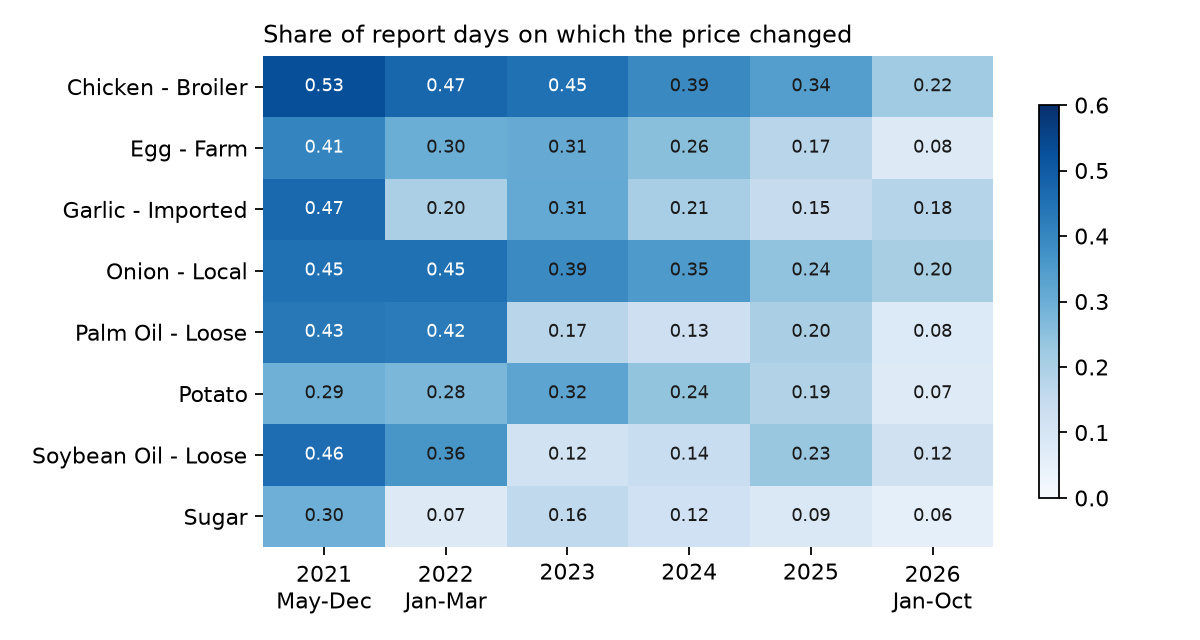
\includegraphics[width=0.9\linewidth]{F1_change_frequency.png}
\caption[Share of report days on which the price changed]{Share of report days on which the price changed, by item and year (2022 covers January to March only, before the gap).}
\label{fig:f1}
\source{\path{reports/figures/F1_change_frequency.png} (notebook 03).}
\end{figure}

This stickiness matters for everything that follows. If the price is unchanged on two days out of three, then ``no change'' is the exact answer on two days out of three, and any model that predicts small movements adds error on those days. The same pattern of infrequent price changes is well documented in studies of retail prices \cite{klenow2010,nakamura2008,cavallo2018}.

\begin{figure}[H]
\centering
\optfig{F2_prices_with_rises.png}{0.95\linewidth}
\caption[Prices of the eight items with sustained rises]{Prices of the eight items with the sustained 10\,\% rises shaded. (This figure shows TCB prices and is kept out of the public repository.)}
\label{fig:f2}
\source{notebook 03, Drive \path{reports/figures/}.}
\end{figure}

\subsection{Sustained rises}
Using the rule of Section~\ref{sec:rise}, the eight items had 70 sustained 10\,\% rises in 2021-26: 11 with onset in 2024 and 23 in 2025-26 (Table~\ref{tab:episodes}). Most of them are in onion (19), potato (18) and imported garlic (12). Palm oil, soybean oil and sugar had no sustained rise in 2024-26, so alerts on these three items cannot be judged as caught or missed; their alerts can only count as unmatched.

\begin{table}[H]\centering\small
\caption[Sustained rise episodes]{Sustained rise episodes by period (onset date), with the 7\,\% and 15\,\% thresholds as a sensitivity check.}\label{tab:episodes}
\fittab{\begin{tabular}{lrrrl}
\toprule
\textbf{Period} & \textbf{7\,\%} & \textbf{10\,\% (main)} & \textbf{15\,\%} & \textbf{Items with no 10\,\% rise} \\
\midrule
2021-26, all & -- & 70 & -- & \\
2024 validation & 17 & 11 & 8 & palm oil, soybean oil, sugar \\
2025-26 \retro & 26 & 23 & 15 & palm oil, soybean oil, sugar \\
\bottomrule
\end{tabular}
}
\source{\path{reports/tables/B5_rise_episodes_by_item_year.csv} (notebook 03).}
\end{table}

\subsection{Before Ramadan}
Table~\ref{tab:ramadan} compares the 30 days before each of the five Ramadans in the data with all other days. Broiler chicken had a positive median change before Ramadan (2.94\,\%) and more rise days (16.1\,\% against 11.1\,\%). Onion and potato had fewer rise days before Ramadan than on other days. The comparison is descriptive: a seasonal pattern is associated with the period and says nothing about why.

\begin{table}[H]\centering\small
\caption[Changes before Ramadan]{Price changes in the 30 days before Ramadan against other days (five Ramadans, about 112 report days per item).}\label{tab:ramadan}
\fittab{\begin{tabular}{lrrrr}
\toprule
 & \multicolumn{2}{c}{\textbf{Median change (\%)}} & \multicolumn{2}{c}{\textbf{Rise days (\%)}} \\
\cmidrule(lr){2-3}\cmidrule(lr){4-5}
\textbf{Item} & before Ramadan & other days & before Ramadan & other days \\
\midrule
Chicken - Broiler & 2.94 & 0 & 16.1 & 11.1 \\
Egg - Farm & $-2.47$ & 0 & 0.0 & 7.3 \\
Garlic - Imported & 0.00 & 0 & 2.7 & 12.7 \\
Onion - Local & $-4.55$ & 0 & 17.9 & 25.2 \\
Palm Oil - Loose & 0.00 & 0 & 3.6 & 0.4 \\
Potato & $-9.76$ & 0 & 8.9 & 24.5 \\
Soybean Oil - Loose & 0.00 & 0 & 0.9 & 0.6 \\
Sugar & 0.00 & 0 & 0.0 & 2.4 \\
\bottomrule
\end{tabular}
}
\source{\path{reports/tables/report/R3_ramadan.csv} (notebook 03).}
\end{table}

\section{Forecast Benchmark (RQ2)}\label{sec:res-forecast}

\subsection{Choice on 2024}
All 16 LightGBM configurations were worse than \naive{} on 2024 (relative MAE 1.047 to 1.536). The simplest one, price history only with 7 leaves, learning rate 0.03 and absolute-error loss, scored best at 1.047 (Table~\ref{tab:grid}). Adding the calendar, weather and exchange-rate drivers made the model worse: the best configuration with drivers scored 1.119. On daily data, these drivers carried no usable signal beyond the recent price path.

\begin{table}[H]\centering\small
\caption[LightGBM configurations on 2024]{LightGBM configurations on 2024 (eight of the sixteen shown, including the best of each feature set; the full grid is in \texttt{M1\_validation\_grid.csv}). Relative MAE is the geometric mean over items of MAE / MAE of \naive{}; above 1 is worse than \naive{}.}\label{tab:grid}
\fittab{\begin{tabular}{llrrrrr}
\toprule
 & & \multicolumn{4}{c}{\textbf{Relative MAE by horizon}} & \\
\cmidrule(lr){3-6}
\textbf{Feature set} & \textbf{Leaves, rate, loss} & 1 & 7 & 14 & 30 & \textbf{All} \\
\midrule
price only & 7, 0.03, l1 (chosen) & 1.114 & 1.029 & 1.035 & 1.014 & \textbf{1.047} \\
price only & 7, 0.05, l1 & 1.219 & 1.033 & 1.062 & 1.040 & 1.086 \\
price only & 31, 0.03, l1 & 1.316 & 1.093 & 1.094 & 1.055 & 1.135 \\
price only & 7, 0.03, huber & 2.098 & 1.134 & 1.072 & 1.001 & 1.264 \\
price + drivers & 7, 0.03, l1 & 1.358 & 1.083 & 1.059 & 1.005 & 1.119 \\
price + drivers & 7, 0.05, l1 & 1.456 & 1.089 & 1.065 & 1.022 & 1.146 \\
price + drivers & 31, 0.03, l1 & 1.617 & 1.165 & 1.145 & 1.080 & 1.236 \\
price + drivers & 7, 0.03, huber & 2.596 & 1.186 & 1.096 & 1.015 & 1.360 \\
\bottomrule
\end{tabular}
}
\source{\path{reports/tables/M1_validation_grid.csv} (notebook 04a, setting committed in \texttt{8d7c145}).}
\end{table}

\subsection{No model beats \naive{}}
Table~\ref{tab:forecast} and Figure~\ref{fig:f3} give the result. Neither ETS nor LightGBM has a relative MAE below 1 at any horizon, in 2024 (1.00 to 1.11) or in 2025-26 (1.01 to 1.21). The gap is largest one day ahead, where \naive{} is right on most days. Where the Diebold--Mariano test finds a significant difference after the Holm correction (3 of 8 comparisons in 2024 and 6 of 8 in 2025-26), the difference is in favour of \naive{}.

The accuracy column shows why accuracy alone would mislead. LightGBM is 99.4\,\% accurate one day ahead in 2025-26, which sounds good, but \naive{} is 99.5\,\% accurate on the same days.

\begin{table}[H]\centering\small
\caption[Forecast benchmark]{Forecast benchmark: MAE of the log change at horizon $h$ (report days), next to \naive{}; relative MAE is the geometric mean over items; Holm $p$ is the corrected Diebold--Mariano $p$-value (``--'': the loss difference has no variance to test).}\label{tab:forecast}
\fittab{\begin{tabular}{llrrrrrr}
\toprule
\textbf{Period} & \textbf{Model} & \textbf{$h$} & \textbf{MAE} & \textbf{MAE naive} & \textbf{Rel.\ MAE} & \textbf{Accuracy} & \textbf{Holm $p$} \\
\midrule
2024 validation & ETS & 1 & 0.009 & 0.009 & 1.060 & 0.991 & 0.003 \\
 & ETS & 7 & 0.032 & 0.032 & 1.010 & 0.968 & 0.027 \\
 & ETS & 14 & 0.051 & 0.051 & 1.004 & 0.948 & 0.146 \\
 & ETS & 30 & 0.083 & 0.083 & 1.002 & 0.914 & 0.281 \\
 & LightGBM & 1 & 0.009 & 0.009 & 1.114 & 0.991 & 0.002 \\
 & LightGBM & 7 & 0.032 & 0.032 & 1.029 & 0.967 & 0.411 \\
 & LightGBM & 14 & 0.052 & 0.051 & 1.035 & 0.947 & 0.434 \\
 & LightGBM & 30 & 0.082 & 0.083 & 1.014 & 0.913 & -- \\
\midrule
2025-26 \retro & ETS & 1 & 0.006 & 0.005 & 1.127 & 0.994 & $<$0.001 \\
 & ETS & 7 & 0.026 & 0.025 & 1.028 & 0.974 & 0.042 \\
 & ETS & 14 & 0.042 & 0.041 & 1.019 & 0.958 & 0.079 \\
 & ETS & 30 & 0.065 & 0.063 & 1.020 & 0.933 & 0.001 \\
 & LightGBM & 1 & 0.006 & 0.005 & 1.213 & 0.994 & $<$0.001 \\
 & LightGBM & 7 & 0.026 & 0.025 & 1.033 & 0.973 & $<$0.001 \\
 & LightGBM & 14 & 0.042 & 0.041 & 1.014 & 0.958 & 0.042 \\
 & LightGBM & 30 & 0.065 & 0.063 & 1.022 & 0.932 & 0.275 \\
\bottomrule
\end{tabular}
}
\source{\path{reports/tables/report/R4_forecast.csv} (notebooks 04a, 04b).}
\end{table}

\begin{figure}[H]
\centering
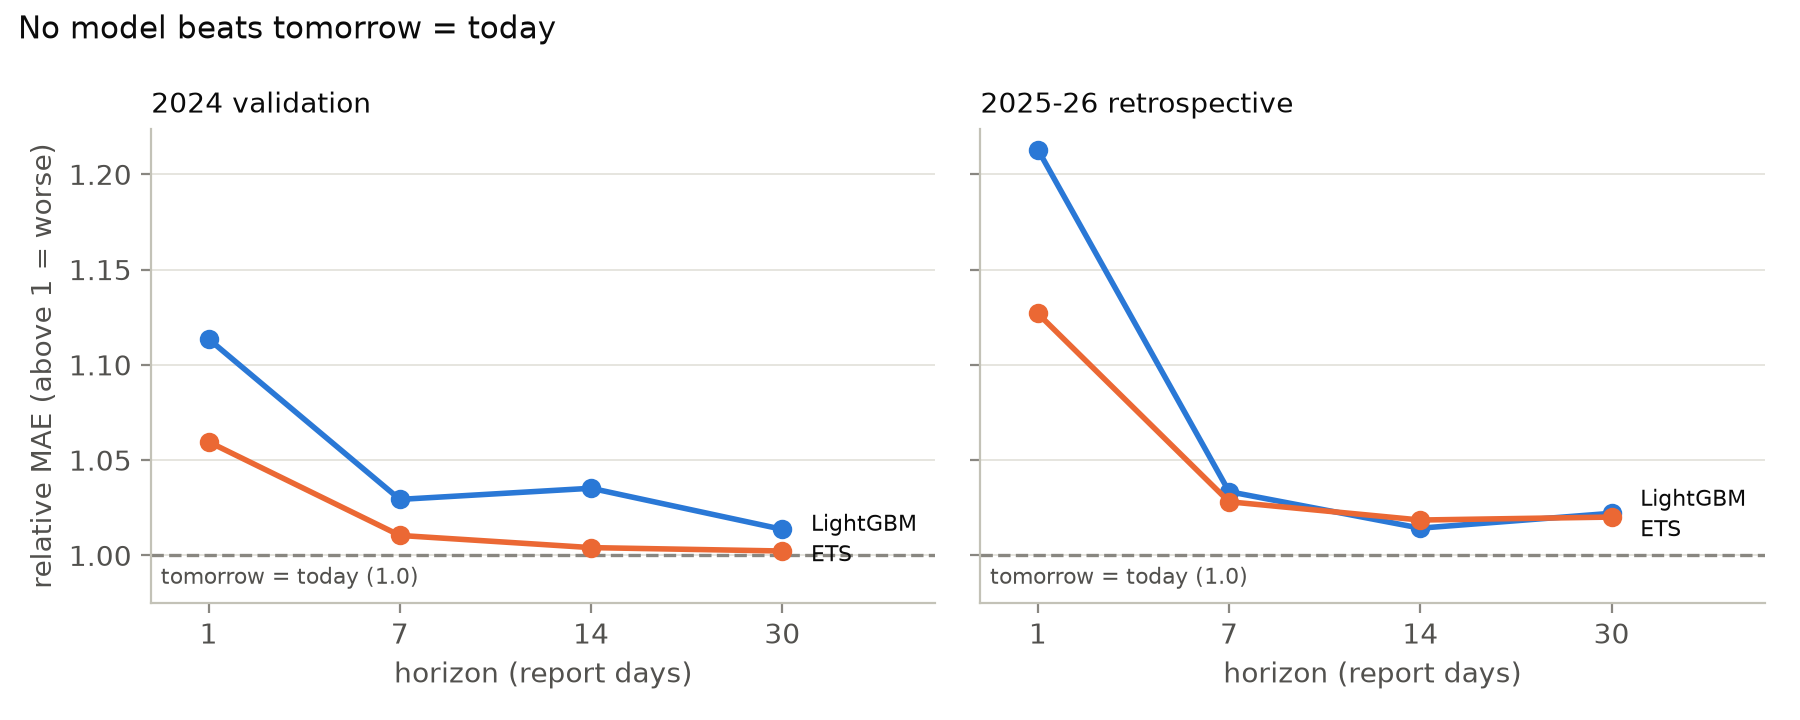
\includegraphics[width=0.85\linewidth]{F3_forecast_vs_naive.png}
\caption[Forecast error relative to \naive{}]{Relative MAE of ETS and LightGBM by horizon; the line at 1 is \naive{}. Every point lies at or above it.}
\label{fig:f3}
\source{\path{reports/figures/F3_forecast_vs_naive.png} (notebook 06).}
\end{figure}

\section{Alert Rules (RQ3, RQ4)}\label{sec:res-alerts}

\subsection{Settings chosen on 2024}
Table~\ref{tab:alertchoice} lists every candidate on 2024. For the ML range (A) and the simple range (B), the 0.90 level gave more than 2 unmatched alert runs per item-year, so the 0.95 level was chosen. For the fixed rise (C), 7\,\% was the most sensitive threshold within the target. These three settings were committed in \texttt{e0cfa06} before any rule was scored on 2025-26.

\begin{table}[H]\centering\small
\caption[Alert settings on 2024]{Alert settings on 2024 (11 sustained rises, 10.53 item-years). The chosen setting is the most sensitive one with at most 2 unmatched alert runs per item-year.}\label{tab:alertchoice}
\fittab{\begin{tabular}{llrrrrl}
\toprule
\textbf{Rule} & \textbf{Setting} & \textbf{Caught} & \textbf{Runs} & \textbf{Precision} & \textbf{Unmatched / item-year} & \textbf{Chosen} \\
\midrule
A. ML range & 0.90 & 9/11 & 39 & 0.23 & 2.85 & \\
 & 0.95 & 6/11 & 17 & 0.35 & 1.04 & yes \\
 & 0.975 & 5/11 & 13 & 0.38 & 0.76 & \\
 & 0.99 & 4/11 & 10 & 0.40 & 0.57 & \\
\midrule
B. Simple range & 0.90 & 9/11 & 36 & 0.25 & 2.56 & \\
 & 0.95 & 8/11 & 20 & 0.40 & 1.14 & yes \\
 & 0.975 & 5/11 & 14 & 0.36 & 0.85 & \\
 & 0.99 & 4/11 & 11 & 0.36 & 0.66 & \\
\midrule
C. Fixed rise & 3\,\% & 10/11 & 58 & 0.17 & 4.56 & \\
 & 5\,\% & 10/11 & 39 & 0.26 & 2.75 & \\
 & 7\,\% & 10/11 & 27 & 0.37 & 1.61 & yes \\
 & 10\,\% & 9/11 & 15 & 0.60 & 0.57 & \\
\bottomrule
\end{tabular}
}
\source{\path{reports/tables/A1_alert_choice.csv} (notebook 05a, committed in \texttt{e0cfa06}).}
\end{table}

\subsection{All three rules beat random dates}
Table~\ref{tab:alertrules} and Figure~\ref{fig:f4} give the scores. In 2024 the ML range caught 6 of 11 sustained rises, the simple range 8 and the fixed rise 10. In 2025-26 \retro{} the ML range caught 17 of 23, the simple range 15 and the fixed rise 22. The same number of alert runs placed on random dates caught far fewer: for the two ranges, the real recall was 2.5 to 2.8 times the random-date recall. In none of the 300 random draws did the random recall reach the real one, for any rule in either period ($p = 0.003$, the smallest value the test can give).

Alerts start a median of 1.5 to 2 report days after a rise begins for the two ranges. This is detection of a rise that is under way, not early warning.

About 6 of every 10 alert runs of the two ranges do not match a sustained 10\,\% rise (precision 0.35 to 0.40). That is roughly 1.0 to 1.3 unmatched runs per item per year. An alert means that the price is unusually high for that item; not every unusual rise goes on to last long enough to count as a sustained 10\,\% rise.

\begin{table}[H]\centering\small
\caption[Alert rules scored against sustained rises]{Alert rules scored against sustained 10\,\% rises. Random = mean recall of the same alert runs on random dates (300 draws); $p$ = random-date $p$-value; Runs = alert runs; Delay = median report days from onset to the matched alert.}\label{tab:alertrules}
\fittab{\begin{tabular}{llrrrrrrr}
\toprule
\textbf{Period} & \textbf{Rule} & \textbf{Caught} & \textbf{Recall} & \textbf{Random} & \textbf{$p$} & \textbf{Runs} & \textbf{Precision} & \textbf{Delay} \\
\midrule
2024 validation & A. ML range & 6/11 & 0.55 & 0.20 & 0.003 & 17 & 0.35 & 1.5 \\
 & B. Simple range & 8/11 & 0.73 & 0.30 & 0.003 & 20 & 0.40 & 2 \\
 & C. Fixed 7\,\% & 10/11 & 0.91 & 0.49 & 0.003 & 27 & 0.37 & 0.5 \\
\midrule
2025-26 \retro & A. ML range & 17/23 & 0.74 & 0.28 & 0.003 & 42 & 0.40 & 2 \\
 & B. Simple range & 15/23 & 0.65 & 0.25 & 0.003 & 39 & 0.38 & 2 \\
 & C. Fixed 7\,\% & 22/23 & 0.96 & 0.31 & 0.003 & 30 & 0.73 & 2 \\
\bottomrule
\end{tabular}
}
\source{\path{reports/tables/report/R5_alert_rules.csv} (notebook 05b).}
\end{table}

\begin{figure}[H]
\centering
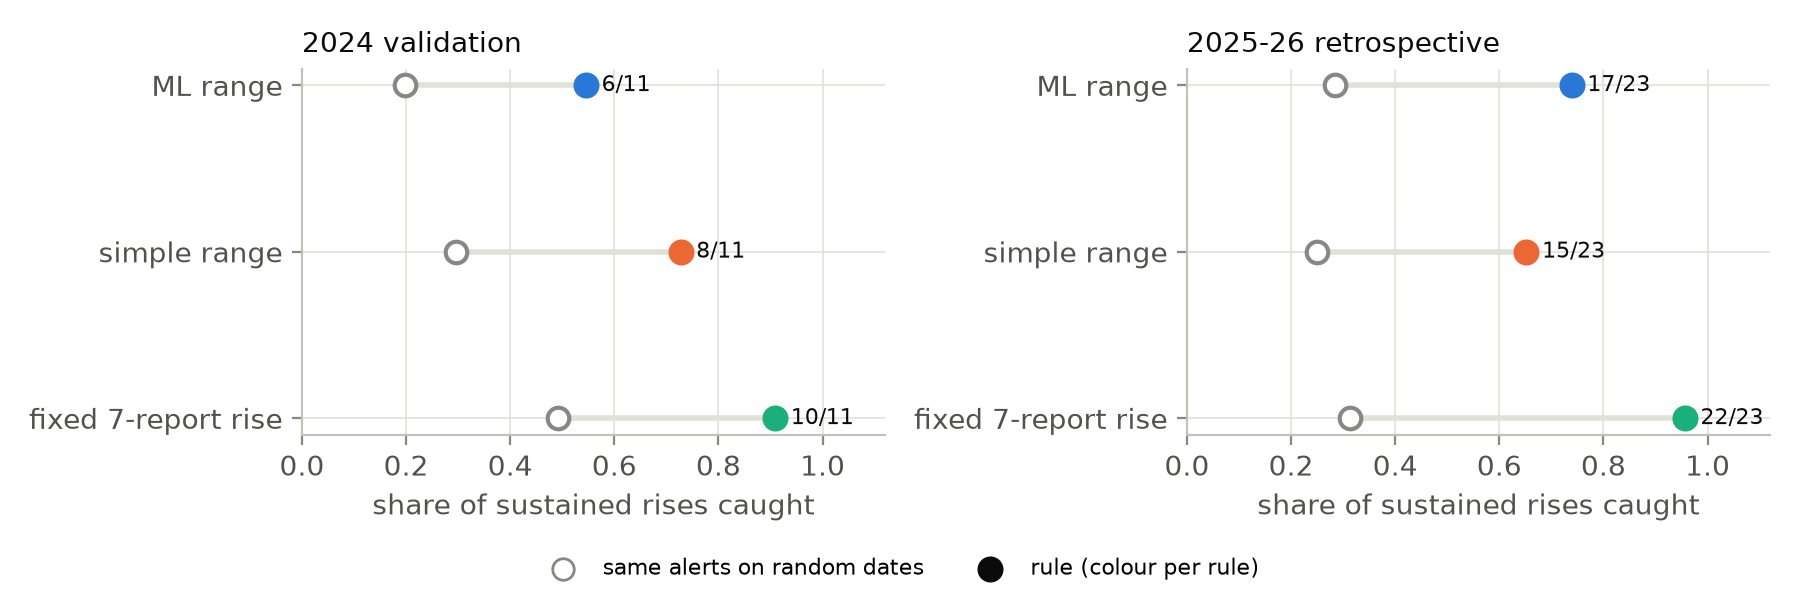
\includegraphics[width=0.85\linewidth]{F4_alert_recall.png}
\caption[Sustained rises caught, against random dates]{Share of sustained rises caught by each rule, against the same alert runs on random dates.}
\label{fig:f4}
\source{\path{reports/figures/F4_alert_recall.png} (notebook 06).}
\end{figure}

\subsection{The ML range adds nothing over the simple range}
The ML range and the simple range catch almost the same rises (Table~\ref{tab:overlap}). In 2024 the simple range caught two rises that the ML range missed and the reverse never happened; in 2025-26 the ML range caught two that the simple range missed and the reverse never happened. Over the two periods each range caught two rises the other missed. This is what Section~\ref{sec:res-forecast} leads one to expect: since the LightGBM forecast is close to \naive{}, the two ranges are close too. For a monitor, the simple range is enough: it catches the same rises and needs no model to be trained or maintained.

\begin{table}[H]\centering\small
\caption[Rises caught by the ML range and the simple range]{Sustained rises caught by the ML range and the simple range.}\label{tab:overlap}
\fittab{\begin{tabular}{lrrrrr}
\toprule
\textbf{Period} & \textbf{Rises} & \textbf{Both} & \textbf{ML range only} & \textbf{Simple range only} & \textbf{Neither} \\
\midrule
2024 validation & 11 & 6 & 0 & 2 & 3 \\
2025-26 \retro & 23 & 15 & 2 & 0 & 6 \\
\bottomrule
\end{tabular}
}
\source{\path{reports/tables/report/R5b_rule_overlap.csv} (notebook 05b).}
\end{table}

\subsection{The fixed rise is a reference, not the winner}
Rule C catches the most rises (10 of 11 and 22 of 23), and in 2025-26 it also has the highest precision. This should not be read as a win. A rise of 7\,\% over 7 report days is very close to the definition of the thing being scored, a rise of 10\,\% over 14 report days lasting 5 days, so its score is partly built in. It also uses one threshold for every item, so it cannot tell an ordinary move of a volatile item such as onion from an unusual move of a stable one. It is reported as a reference point for the two ranges.

\subsection{Results by item}
Table~\ref{tab:byitem} shows each item. Onion, potato and garlic hold most of the rises. On the three items without any sustained rise, the ranges still raised 2 to 5 alert runs per period; these are the unmatched alerts of a sticky price that moved by more than usual.

\begin{table}[H]\centering\small
\caption[Alerts by item]{Rises caught / rises (alert runs) by item and rule. ``--'': no sustained rise in the period, so the alerts cannot be judged.}\label{tab:byitem}
\fittab{\begin{tabular}{lllllll}
\toprule
 & \multicolumn{3}{c}{\textbf{2024 validation}} & \multicolumn{3}{c}{\textbf{2025-26 \retro}} \\
\cmidrule(lr){2-4}\cmidrule(lr){5-7}
\textbf{Item} & A & B & C & A & B & C \\
\midrule
Chicken - Broiler & 1/1 (3) & 1/1 (4) & 1/1 (5) & 1/3 (4) & 1/3 (4) & 2/3 (3) \\
Egg - Farm & 1/1 (1) & 1/1 (1) & 1/1 (3) & 3/3 (7) & 3/3 (6) & 3/3 (4) \\
Garlic - Imported & 1/2 (1) & 1/2 (1) & 1/2 (1) & 4/4 (7) & 4/4 (8) & 4/4 (7) \\
Onion - Local & 2/4 (2) & 3/4 (3) & 4/4 (10) & 5/7 (6) & 5/7 (6) & 7/7 (9) \\
Potato & 1/3 (2) & 2/3 (3) & 3/3 (8) & 4/6 (5) & 2/6 (3) & 6/6 (6) \\
Palm Oil - Loose & -- (3) & -- (3) & -- (0) & -- (4) & -- (4) & -- (0) \\
Soybean Oil - Loose & -- (3) & -- (3) & -- (0) & -- (4) & -- (3) & -- (0) \\
Sugar & -- (2) & -- (2) & -- (0) & -- (5) & -- (5) & -- (1) \\
\bottomrule
\end{tabular}
}
\source{\path{reports/tables/report/R6_focus_items.csv} (notebook 05b).}
\end{table}

\subsection{Range coverage}
A 95\,\% upper bound should hold the price on about 95\,\% of days. In 2024 it did: 94.5\,\% for the ML range and 94.6\,\% for the simple range, consistent with 95\,\% by Kupiec's test (Table~\ref{tab:coverage}). In 2025-26 coverage was 93.4\,\% and 93.9\,\%, slightly but significantly below 95\,\%. A range built from the last 120 errors adapts slowly when prices become more volatile.

\begin{table}[H]\centering\small
\caption[Coverage of the expected range]{Share of days at or below the upper bound, against the nominal 95\,\%, with Kupiec's test.}\label{tab:coverage}
\fittab{\begin{tabular}{llrrrr}
\toprule
\textbf{Period} & \textbf{Rule} & \textbf{Days} & \textbf{Nominal} & \textbf{Coverage} & \textbf{Kupiec $p$} \\
\midrule
2024 validation & A. ML range & 2632 & 0.95 & 0.945 & 0.205 \\
 & B. Simple range & 2632 & 0.95 & 0.946 & 0.358 \\
2025-26 \retro & A. ML range & 4824 & 0.95 & 0.934 & $<$0.001 \\
 & B. Simple range & 4824 & 0.95 & 0.939 & 0.001 \\
\bottomrule
\end{tabular}
}
\source{\path{reports/tables/report/R7_range_coverage.csv} (notebook 05b).}
\end{table}

\section{Sample Input and Output}\label{sec:res-monitor}
This section follows one real case through the system, in the order in which the system processes it: the sustained rise of local onion that began on 2 November 2025 (2025-26, retrospective). The rise lasted 16 report days, to 17 November 2025, with a peak rise of 57\,\% over 14 report days.

\subsection{Input}
The input on each report day is the TCB row of the item, joined with its drivers (Table~\ref{tab:datasample}), and the 7-day forecast made one week earlier. For onion, the drivers are the weather columns; the chosen LightGBM uses price history only.

\subsection{Expected range}
On each day $t$, the upper bound of the ML range is the LightGBM forecast made at $t-7$ plus the 95th percentile of onion's last 120 forecast errors known at $t-7$. The bound is fixed before day $t$ is seen.

\subsection{Alert decision}
Table~\ref{tab:worked} follows the days around the onset. Onion was above the bound on the onset day and the next day, which is not yet an alert. On 4 November 2025, the third day above the bound in the last five, the alert run started: 2 report days after the onset.

\begin{table}[H]\centering\footnotesize
\caption[Worked example: onion, November 2025]{Worked example: local onion around the onset of the rise of 2 November 2025, under the ML range (prices in Tk; change over 7 report days).}\label{tab:worked}
\opttab{worked_example}
\source{\texttt{processed/monitor\_8.csv} on Drive (contains prices; not in the public repository).}
\end{table}

\subsection{Output in the app}
Figures~\ref{fig:app-status} to \ref{fig:app-how} show the four tabs of the app for this case.

\begin{figure}[H]
\centering
\optfig[245 30 245 0]{monitor_status.png}{\linewidth}
\caption[App: status on a day]{App, ``Status on a day'': all eight items on 4 November 2025 under the ML range; onion is in alert.}
\label{fig:app-status}
\end{figure}

\begin{figure}[H]
\centering
\optfig[240 10 255 0]{monitor_item.png}{\linewidth}
\caption[App: item chart]{App, ``Item'': onion from October to November 2025 with the upper bound, the sustained rise shaded and the start of the alert run.}
\label{fig:app-item}
\end{figure}

\begin{figure}[H]
\centering
\optfig[310 45 310 0]{monitor_log.png}{\linewidth}
\caption[App: alert log]{App, ``Alert log'': alert runs of the ML range in 2025-26 with the hindsight match.}
\label{fig:app-log}
\end{figure}

\begin{figure}[H]
\centering
\optfig{monitor_how.png}{\linewidth}
\caption[App: how it works]{App, ``How it works'': the three rules and their scores.}
\label{fig:app-how}
\end{figure}

\subsection{Validation}
In hindsight, the alert run that started on 4 November 2025 lies inside the match window of the rise (14 report days before the onset to 7 after its end), so it counts as a caught rise in Table~\ref{tab:alertrules}. For the whole period, the app's alert flags were checked to be identical to those scored in notebook 05b, and its counts of alert runs equal Table~\ref{tab:alertrules}. Figure~\ref{fig:f5} shows the alerts of the three rules on onion, potato and egg over 2024-26.

\begin{figure}[H]
\centering
\optfig{F5_prices_with_alerts.png}{0.95\linewidth}
\caption[Prices with alerts for onion, potato and egg]{Onion, potato and egg prices, 2024 to October 2026, with sustained rises shaded and the start of each alert run of the three rules.}
\label{fig:f5}
\source{notebook 06, Drive \path{reports/figures/}.}
\end{figure}


\section{Discussion}

\subsection{Why \naive{} wins}
The forecast result follows from the price behaviour. TCB records a price that is unchanged on 62 to 87\,\% of report days and that moves in steps of at least Tk 0.5. On such a series, the last price is the best guess most of the time. A model that learns average movements from history spreads small predicted changes over many days on which nothing happens, and loses more on those days than it gains on the few days with a large move. This is the same lesson as the long line of studies in which the random walk is hard to beat out of sample \cite{meese1983}, and it matches the Bangladeshi benchmark in which naive persistence won on commodities that behave like a random walk \cite{agripricebd}. The drivers did not help because, on a daily scale, weather and the exchange rate change slowly and are already reflected in the recent price path.

\subsection{What the alerts can and cannot say}
The alerts work: all three rules catch far more sustained rises than the same number of alerts on random dates, and the ranges do so a median of 1.5 to 2 report days after a rise begins. An alert says that the price of an item has stayed above what its own recent behaviour would lead one to expect. Such a rise is \unexpl{} in this system. The alert does not say why the price rose; finding that out needs other evidence.

\subsection{Which rule to use}
The ML range and the simple range catch nearly the same rises, so the machine-learning model adds nothing to the alerts. For a monitor that someone has to keep running, the simple range is the better choice: same rises, no model to train, and a rule that is easy to explain. The app shows the ML range first so that the comparison stays visible, and it states this finding beside it.

\section{Threats to Validity}\label{sec:threats}
\begin{itemize}[leftmargin=*,itemsep=2pt]
\item \textbf{Retrospective test period.} 2025-26 had been looked at by an earlier run of the project. No setting in this run was chosen on it, and the commits show the order, but the design of the comparison was made after those earlier results were known.
\item \textbf{Item choice.} The eight items were chosen after the earlier 54-item results had been seen.
\item \textbf{Few rises.} 2024 has 11 sustained rises and 2025-26 has 23. Rates are always shown with their counts. The random-date test does not need large samples, and both periods point the same way.
\item \textbf{Three items without rises.} For palm oil, soybean oil and sugar, recall cannot be measured.
\item \textbf{Rule C is partly circular}, as discussed above.
\item \textbf{The reference is a definition.} A sustained 10\,\% rise over 14 report days is one reasonable definition among several; the 7\,\% and 15\,\% counts show how much it matters.
\item \textbf{Data.} The audit confirms the copying of the TCB sheets, not the accuracy of what TCB recorded. TCB reports a range for Dhaka markets, and the midpoint is used as the price.
\item \textbf{Coverage} in 2025-26 is slightly below its nominal level.
\end{itemize}

\chapter{Conclusion, Limitations and Future Work}\label{ch:concl}

\section{Conclusion}
This project built Food Price Watch, a monitoring and abnormal-rise alert system for the TCB daily retail prices of eight food items in Dhaka, and evaluated it with every setting chosen on 2024 and committed before 2025-26 was scored. The prices are sticky: an item's price is unchanged on 62 to 87\,\% of report days, yet sustained 10\,\% rises do happen (70 in 2021-26), mostly in onion, potato and imported garlic (RQ1). Neither ETS nor LightGBM beats \naive{} at any horizon, in 2024 (relative MAE 1.00 to 1.11) or in 2025-26 \retro{} (1.01 to 1.21), and every significant difference favours \naive{} (RQ2). The alerts do catch sustained rises: the ML range caught 6 of 11 in 2024 and 17 of 23 in 2025-26 \retro{}, and the simple range 8 of 11 and 15 of 23, about 2.5 to 2.8 times the recall of the same alerts on random dates ($p = 0.003$), a median of 1.5 to 2 report days after a rise begins (RQ3). The two ranges catch nearly the same rises, so a daily monitor for these prices does not need machine learning: a range drawn from each item's own past price changes is enough (RQ4).

\section{Limitations}
\begin{itemize}[leftmargin=*,itemsep=2pt]
\item The 2025-26 results are retrospective: that period had been looked at in an earlier run of the project.
\item The eight items were chosen after the earlier results had been seen.
\item There are few sustained rises (11 in 2024, 23 in 2025-26), and none for three of the items.
\item Rule C is close to the definition of a sustained rise, so its score is partly circular.
\item The range was slightly too narrow in 2025-26 (coverage 93.4 to 93.9\,\% against 95\,\%).
\item Only rises are monitored; only Dhaka is covered; and the monitor replays past data rather than receiving new sheets.
\item The price is the midpoint of TCB's lowest and highest price, and its accuracy depends on TCB's own recording.
\end{itemize}

\section{Future Work}
\begin{itemize}[leftmargin=*,itemsep=2pt]
\item Connect the monitor to new TCB sheets as they are published, with TCB's permission, and run it forward on genuinely unseen days.
\item Extend it to more items, to falls as well as rises, and to other cities.
\item Make the range adapt faster when an item becomes more volatile, to bring coverage back to its nominal level.
\item Compare the alerts with FAO's and WFP's indicators on the same items, and test whether weekly or monthly drivers help at longer horizons.
\end{itemize}


% ============================ REFERENCES ============================
\clearpage
\addcontentsline{toc}{chapter}{\numberline{}References}
\renewcommand{\bibname}{References}
\bibliographystyle{unsrt}
\bibliography{ref}

% ============================ APPENDICES ============================
\appendix
\chapter{Reproducibility Record}\label{app:repro}
The code is in the public repository \url{https://github.com/mrchowdhury587/foodprice_watch}. Each notebook clones the code, runs on the data folder, and prints its code commit and the sha256 hashes of its inputs and outputs. Notebooks 02 to 06 were run on the work computer and again in Google Colab; every output was byte-identical (Table~\ref{tab:repro}).

\begin{table}[H]\centering\small
\caption[Output files and their hashes]{Main output files and the first eight characters of their sha256 hash, identical in the local and the Colab runs.}\label{tab:repro}
\fittab{\begin{tabular}{lll}
\toprule
\textbf{File} & \textbf{Written by} & \textbf{sha256 (first 8)} \\
\midrule
\texttt{data\_8.csv} & 02 processing & 381ef71d \\
\texttt{rise\_episodes\_8.csv} & 03 price behaviour & 48d529fc \\
\texttt{forecasts\_test.csv} & 04b forecast test & d536b503 \\
\texttt{forecasts\_h7.csv} & 04b forecast test & 6449ec4d \\
\texttt{alerts\_8.csv} & 05b alert scoring & 613b3c45 \\
\texttt{R1\_data.csv} & 06 report tables & 63cafc13 \\
\bottomrule
\end{tabular}
}
\source{\path{reports/RUN_LOG.md}.}
\end{table}

\begin{table}[H]\centering\small
\caption[Commits that fixed the settings]{Commits that fixed the settings before scoring.}\label{tab:commits}
\begin{adjustbox}{max width=\linewidth}\begin{tabular}{lll}
\toprule
\textbf{Commit} & \textbf{What was fixed} & \textbf{Before} \\
\midrule
\texttt{8d7c145} & LightGBM: price only, 7 leaves, rate 0.03, absolute-error loss & notebook 04b (forecast test) \\
\texttt{e0cfa06} & alert settings: ML range 0.95, simple range 0.95, fixed rise 7\,\% & notebook 05b (alert scoring) \\
\bottomrule
\end{tabular}\end{adjustbox}
\end{table}

\chapter{Results Register}\label{app:register}
Every headline number of this report is listed in \path{reports/RESULTS_REGISTER.md} with the committed table it comes from, the notebook that wrote the table, and the commit. Results for 2025-26 carry the label ``retrospective''.

\chapter{Changes to the Original Plan}\label{app:deviations}
Every change to items, dates, drivers, method, thresholds or sources was written into \path{DEVIATIONS.md} before work continued. The list below covers every entry; the file gives the reasons and approvals.
\begin{itemize}[leftmargin=*,itemsep=2pt]
\item \textbf{Scope.} The project was restarted under the present title. The earlier pipeline stays unchanged in the archive. The forecasts became a benchmark and the monitoring and alert system became the product, because the earlier model had not beaten \naive{}.
\item \textbf{Items.} Eight items instead of 54, chosen for how often their prices move and for being everyday purchases, after the earlier results had been seen (Section~\ref{sec:threats}).
\item \textbf{Drivers.} Kept: calendar, exchange rate and weather. Dropped: the India onion export flag (its source ends in March 2025), public holidays (the Eids are in the Ramadan--Eid file) and news events.
\item \textbf{Exchange rate.} One source only (Yahoo), without the earlier splice. The 30-day change now takes the last quote on or before the day 30 days earlier (at most 7 days older); looking up that exact day had left 28\,\% of values empty. The Yahoo series is stale from about September 2026, so the 30-day change is understated in the last weeks.
\item \textbf{Data files.} Four raw files; the item list moved into the settings file; the panel and feature files were merged into one table of 20 columns with no change of values.
\item \textbf{Forecast.} Three candidates (\naive{}, ETS, LightGBM) instead of six; LightGBM chosen from a 16-configuration grid on 2024 instead of a 50-trial search; 82 weekly test origins whose 30-day target lies on or before 24 October 2026.
\item \textbf{Alerts.} Each rule's setting is the most sensitive candidate whose 2024 alert runs that match no sustained rise stay at or below 2 per item-year; the earlier run counted alerts outside news-event windows, which were dropped.
\item \textbf{Test period.} 2025-26 had been scored by the earlier run, so every result on it is labelled retrospective; all choices were still made on 2024.
\item \textbf{Plan claims not met.} Alerts catch 55 to 74\,\% of rises (plan: 65 to 75\,\%), 2.5 to 2.8 times the random-date rate (plan: about three), with three forecast models (plan: six). Two-sided range coverage is not reported because the ranges are upper bounds only.
\item \textbf{Runs.} Notebooks 03 to 06 were first run on the work computer while Google Drive could not be mounted in Colab, then rerun in Colab with identical outputs; the Colab runs are the runs of record.
\item \textbf{Monitor.} Notebook 07 and the Gradio app replay the three rules to 24 October 2026. The app can be shared through a temporary public link, approved by the project owner.
\item \textbf{Report.} This report replaces the earlier one on the same university template: new title and four research questions; the driver-breakdown and news-event chapters were dropped.
\end{itemize}


\end{document}
